\documentclass[../Article_Sensitivity_Analsysis.tex]{subfiles}
\graphicspath{{\subfix{../Figures/}}}
\begin{document}
	
    %\subsection{Pressure}
	
	As discussed in Chapter \ref{CH:Governing_equations_chapter}, a small pressure wave propagates at the speed of sound relative to the flow. When the flow velocity is relatively low, pressure changes are hydrodynamic (resulting from velocity motion) rather than thermodynamic. The Low Mach number assumption allows for the instant propagation of thermodynamic pressure throughout the system, enabling a single pressure value to be considered for the entire system. In response to a pressure change, the energy equation experiences a simultaneous deviation across the entire spatial domain. This pressure change impacts the fluid's temperature within the computational domain, while boundary values are constrained by conditions specified at the domain's extremes. Dirichlet boundary conditions impose a fixed temperature value at the inlet, creating a thermal gradient that propagates through the system. On the other hand, Neumann boundary conditions specify the heat flux at the boundaries. In this study, zero Neumann boundary conditions were applied to ensure that the temperatures at the inlet, outlet, and within the extractor vary uniformly in response to the pressure change.
	
	Figure \ref{fig:Sensitivty_P_CS} illustrates the sensitivity of solute concentration in the solid phase to pressure changes. As discussed in Chapter \ref{CH: Continuity}, the velocity of a fluid is inversely proportional to its density, indicating that increased pressure reduces the fluid's velocity. This results in an extended residence time, allowing for longer interaction between the solute and solvent.	Initially, the extraction process operates in the kinetic-controlled regime, where the concentration gradient is high, and solute solubility is the limiting factor. As noted in [article 1], the system is considered far from saturation, which explains the low initial system response. This low initial response was also observed in the sensitivity analysis by \citet{Fiori_2007}. The system's response becomes more pronounced as the concentration gradient decreases and the extraction shifts from the kinetic-controlled to the diffusion-controlled regime. The negative sensitivity indicates a faster solute loss from the solid phase, corresponding to enhanced mass transfer.  Over time, as the amount of solute decreases, it becomes a limiting factor, reducing the effect of pressure changes on the system. Eventually, the sensitivities approach zero asymptotically as the solute is washed out from the bed.

	\begin{figure}[!ht]
		\centering
		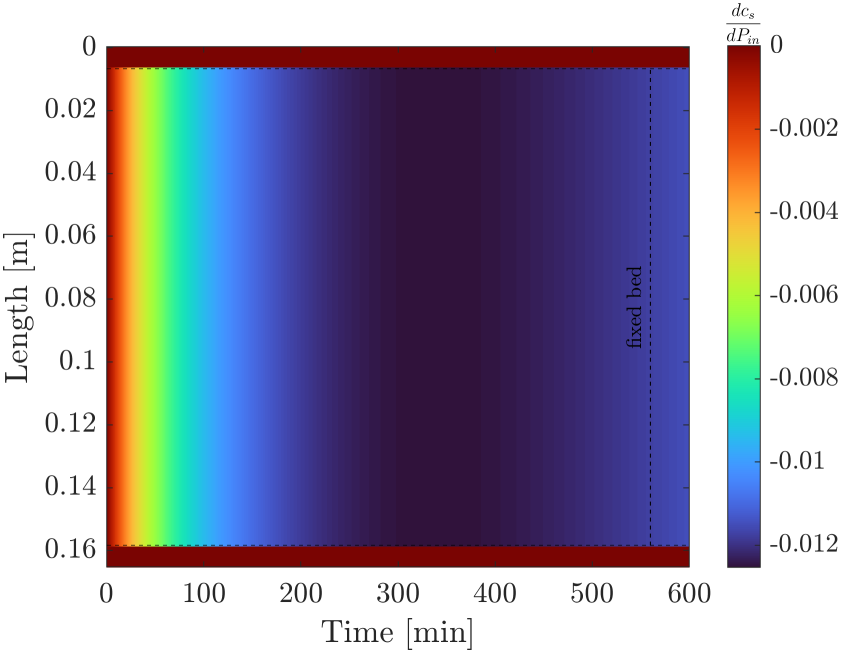
\includegraphics[trim = 0.0cm 0.0cm 0.0cm 0.0cm,clip,width=\columnwidth]{/Results_sensitivity/CS_P_1.png}
		\caption{The effect of $P_{in}$ change on $C_s$}
		\label{fig:Sensitivty_P_CS}
	\end{figure}

	Figure \ref{fig:Sensitivty_P_CF} illustrates the sensitivity of solute concentration in the fluid phase to pressure changes. Compared to Figure \ref{fig:Sensitivty_P_CS}, the dynamic behaviour of fluid phase sensitivities is more apparent. Due to advection, the sensitivities move through the system similarly to the solute in the fluid phase.	Initially, the system response is low despite the pressure increase improving mass transfer, reflecting the previously discussed idle period. As the process continues, the sensitivities increase, indicating faster solute loss from the solid phase. The positive sensitivities show that more solute is being transported from the solid particles to the fluid. When the solute in the solid phase becomes a limiting factor, the extraction rate slows, and sensitivities decline to negative values, eventually approaching zero asymptotically.
	
	\begin{figure}[!ht]
		\centering
		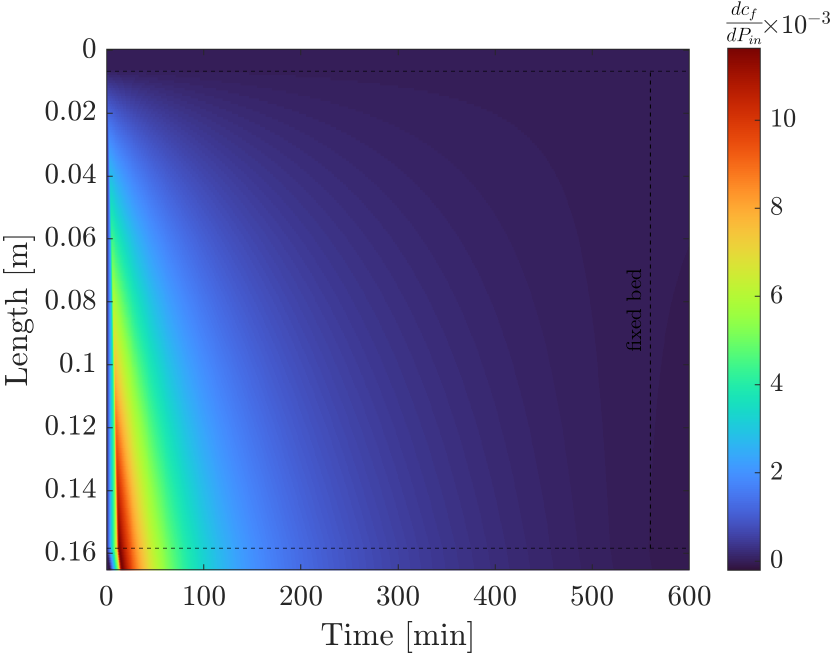
\includegraphics[trim = 0.0cm 0.0cm 0.0cm 0.0cm,clip,width=\columnwidth]{/Results_sensitivity/CF_P_1.png}
		\caption{The effect of $P_{in}$ change on $C_f$}
		\label{fig:Sensitivty_P_CF}
	\end{figure}
	
	Figure \ref{fig:Sensitivty_P_y} show how sensitive the extraction yield is to pressure changes over an extended period for various pressure values. Initially, all sensitivity curves remain nearly flat, indicating a delayed response in the system. Due to the reduced fluid velocity, the solute reaches the extractor's outlet later, causing minor negative sensitivities to appear. Once the solute exits the extractor, the sensitivity curves rise. Positive yield sensitivities indicate improved process efficiency and enhanced mass transfer. The peak in $\frac{dy}{dP_{in}}$ represents the point of greatest deviation from the original system. Eventually, the sensitivities decline and converge towards zero as the concentration gradient becomes a limiting factor, reducing the impact of enhanced mass transfer.
	
	As presented in Figure \ref{fig:Sensitivty_P_y}, higher sensitivities are observed for the low-pressure system. At lower pressures, the supercritical fluid has lower density and solvating power, which results in less efficient extraction as shown by data given in {\color{red}article 1}. Small changes in pressure at low pressures can significantly impact the solute's solubility and, consequently, the extraction yield. Moreover, near the critical point, small changes in pressure can lead to significant changes in the physical properties of the supercritical fluid, such as density and viscosity and consequently to higher sensitivity of the system state-space.
	
	\begin{figure}[!ht]
		\centering
		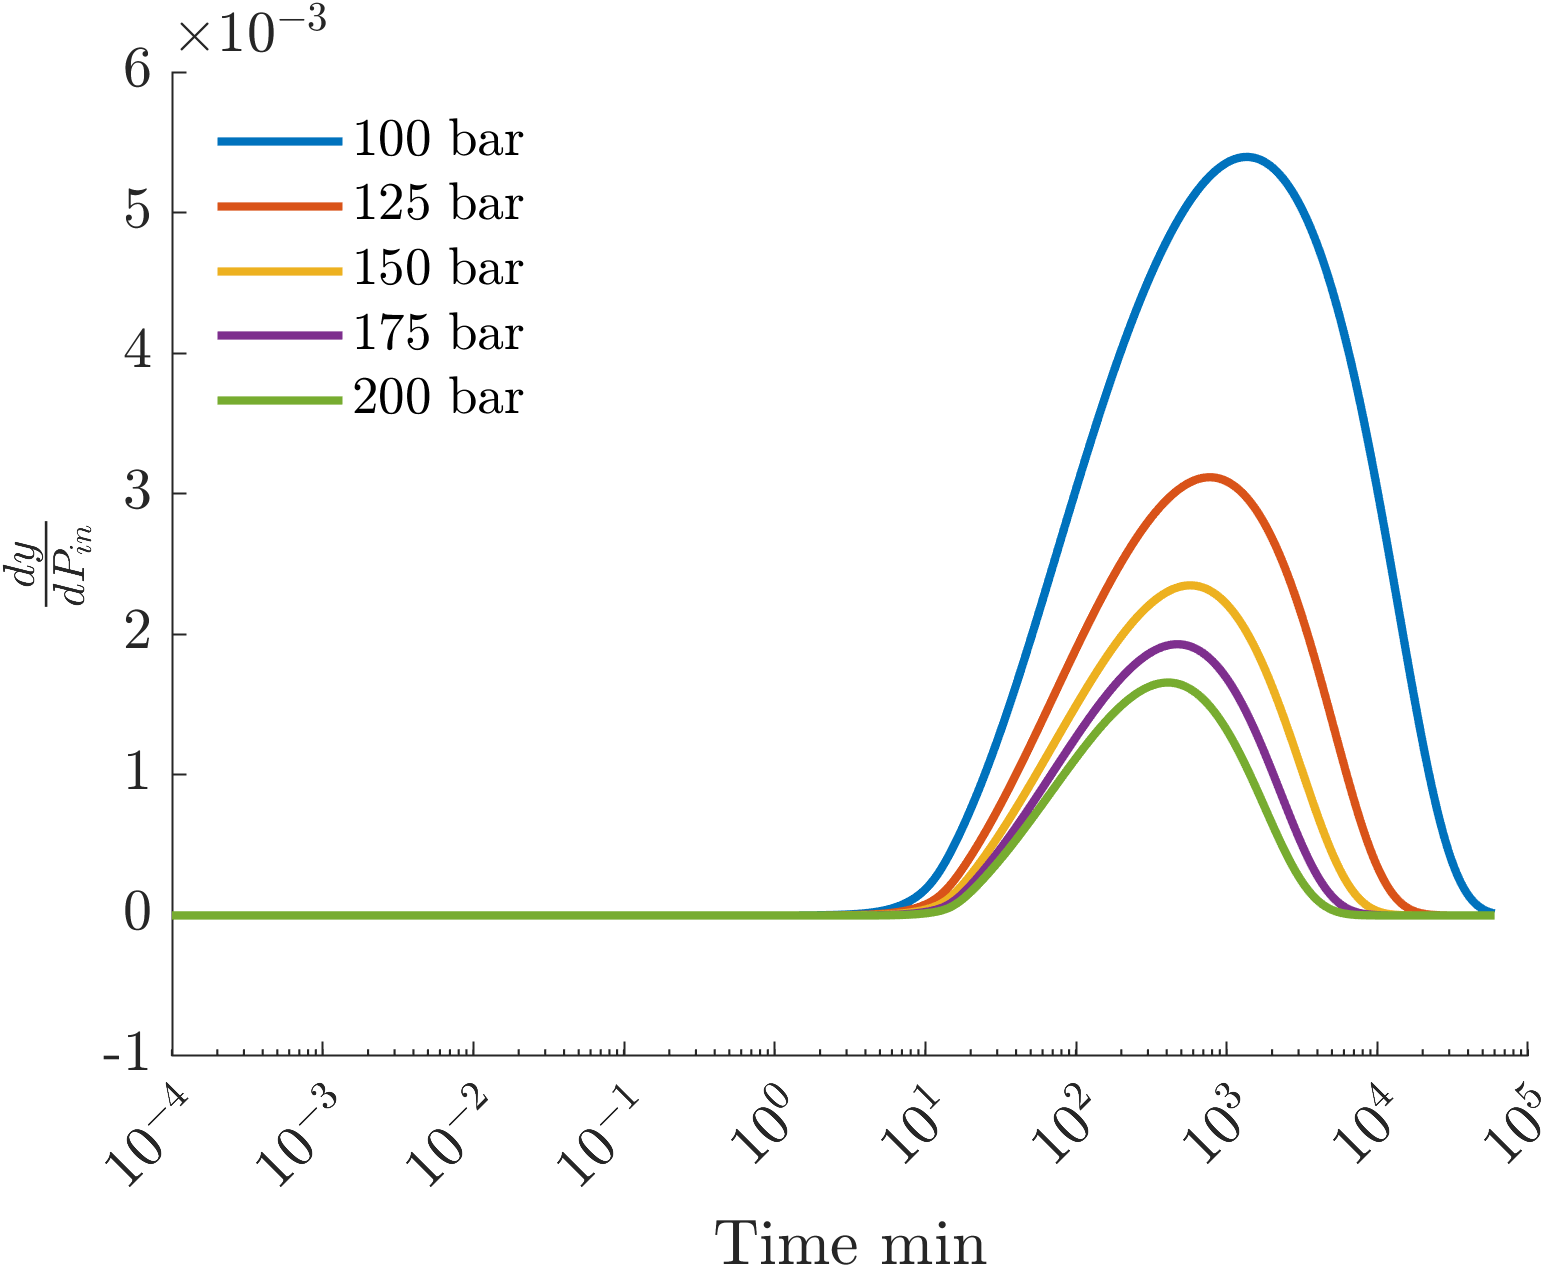
\includegraphics[trim = 0.1cm 0.0cm 1.0cm 0.0cm,clip,width=\columnwidth]{/Results_sensitivity/Yield_Multiple.png}
		\caption{The effect of $P_{in}$ change on $y(t)$}
		\label{fig:Sensitivty_P_y}
	\end{figure}
		
\end{document}


































